\documentclass[tikz,border=12pt]{standalone}
% Shared visual language for standalone EMT block diagrams.
\usepackage{amsmath}
\usetikzlibrary{arrows.meta,backgrounds,calc,fit,positioning}

\tikzset{
    emt diagram/.style = {>={Stealth[length=2.4mm]}},
    line/.style        = {semithick, rounded corners=6pt},
    block/.style       = {draw, semithick, fill=white,
                          minimum height=1cm, minimum width=2.3cm},
    hblock/.style      = {block, minimum width=2.24cm, minimum height=1.3cm},
    vblock/.style      = {block, minimum width=1.3cm, minimum height=2.24cm},
    sum/.style         = {draw, semithick, fill=white, circle,
                          inner sep=2.6pt},
    signal/.style      = {circle, fill, inner sep=1.4pt,
                          label distance=3pt},
    sig/.style         = {font=\small},
    pm/.style          = {font=\scriptsize},
    wire jump/.style   = {line,
                          preaction={draw=white, line width=3pt,
                                     line cap=round}},
    enclosure/.style   = {draw, dashed, semithick, rounded corners=4pt},
    operator enclosure/.style = {enclosure, inner xsep=7mm, inner ysep=6mm}
}


% TUNABLES: gain width, integral branch height, and angle feedback height.
\def\gainwidth{1.35cm}
\def\integralrow{-2.2}
\def\feedbackrow{-3.8}

\begin{document}
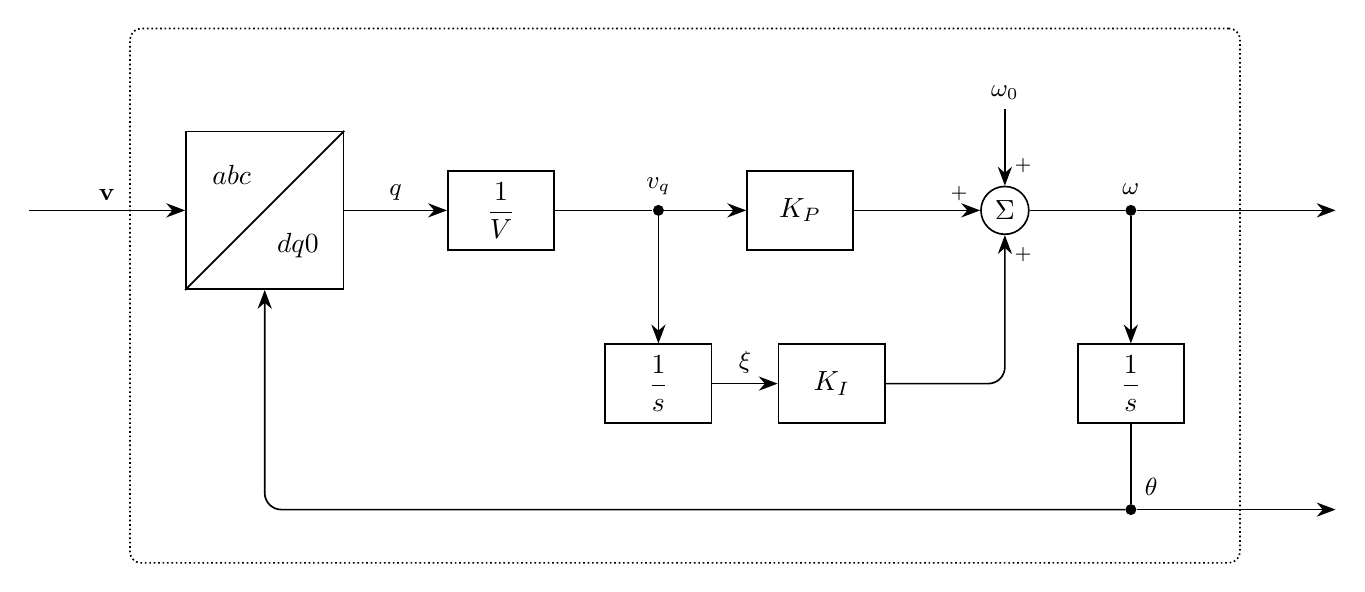
\begin{tikzpicture}[emt diagram]

% Power-invariant Park transformation; only the q coordinate is used.
\node[block, minimum width=2cm, minimum height=2cm] (park) at (0,0) {};
\draw[semithick] (park.south west) -- (park.north east);
\node at ($(park.center)+(-0.42,0.45)$) {$abc$};
\node at ($(park.center)+(0.42,-0.45)$) {$dq0$};
\node[block, minimum width=\gainwidth] (normalization)
    at (3,0) {$\dfrac{1}{V}$};
\node[signal, label={[sig]above:$v_q$}] (vq) at (5,0) {};
\draw[->, line] (-3,0) -- node[sig, above] {$\mathbf{v}$} (park.west);
\draw[->, line] (park.east) -- node[sig, above] {$q$} (normalization.west);
\draw[line] (normalization.east) -- (vq);

% Proportional and integral frequency corrections.
\node[block, minimum width=\gainwidth] (Kp) at (6.8,0) {$K_P$};
\node[sum] (sum) at (9.4,0) {$\Sigma$};
\node[sig] (nominal) at (9.4,1.5) {$\omega_0$};
\node[block, minimum width=\gainwidth] (xi)
    at (5,\integralrow) {$\dfrac{1}{s}$};
\node[block, minimum width=\gainwidth] (Ki)
    at (7.2,\integralrow) {$K_I$};
\draw[->, line] (vq) -- (Kp.west);
\draw[->, line] (Kp.east) -- (sum.west);
\node[pm, above left=0pt and 1pt of sum.west] {$+$};
\draw[->, line] (nominal.south) -- (sum.north);
\node[pm, above right=1pt and 0pt of sum.north] {$+$};
\draw[->, line] (vq) -- (xi.north);
\draw[->, line] (xi.east) -- node[sig, above] {$\xi$} (Ki.west);
\draw[->, line] (Ki.east) -| (sum.south);
\node[pm, below right=1pt and 0pt of sum.south] {$+$};

% Frequency and angle outputs share a vertical integration path.
\node[signal, label={[sig]above:$\omega$}] (omega) at (11,0) {};
\node[block, minimum width=\gainwidth] (integrator)
    at (11,\integralrow) {$\dfrac{1}{s}$};
\node[signal, label={[sig]above right:$\theta$}]
    (theta) at (11,\feedbackrow) {};
\coordinate (feedback) at (0,\feedbackrow);
\draw[line] (sum.east) -- (omega);
\draw[->, line] (omega) -- (13.6,0);
\draw[->, line] (omega) -- (integrator.north);
\draw[line] (integrator.south) -- (theta);
\draw[->, line] (theta) -- (13.6,\feedbackrow);
\draw[->, line] (theta) -- (feedback) -- (park.south);

% Enclose the model-owned states, variables, and feedback paths.
\begin{scope}[on background layer]
    \node[operator enclosure, densely dotted,
        fit=(park)(normalization)(vq)(Kp)(sum)(nominal)
            (xi)(Ki)(omega)(integrator)(theta)(feedback)] {};
\end{scope}

\end{tikzpicture}
\end{document}
